\section{실험 결과}
\label{sec:results}

\subsection{R1 진단과 최소 학습}

기본 CoC 대비 문장 추가에 따른 2초 trajectory 변화는 약 $+0.263$ m였으나 hold와 반대 의미 Guard 사이 차이는 약 $0.008$ m였다. 따라서 R1 trajectory가 CoC 문장 변화에 반응한다는 증거는 있지만, 반대 의미를 안정적으로 구별한 zero-shot 준수 증거는 약했다. 이를 "약한 방향성 반응은 있으나 의미 특이성은 확인되지 않음"으로 판정하였다.

최소 Guard 학습에서 올바른 Guard pair 조건은 held-out 정확도 0.990과 동일 장면 counterfactual 완전 정답률 0.958을 기록했고, shuffled 조건은 각각 0.719와 0.000이었다. 그러나 paraphrase 정확도는 0.740 대 0.745였고 두 조건의 paraphrase pair가 모두 0이었다. 이는 in-distribution Guard--행동 대응은 학습 가능하지만 표현 일반화는 확립되지 않았음을 뜻한다.

충분한 학습량의 쉬운 STOP/PROCEED 과제에서는 Traditional CoC도 held-out 0.974, pair 0.896에 도달했고 CoC+Guard는 1.000, 1.000이었다. Equal-step 사후 진단에서는 두 조건 모두 held-out와 pair가 1.000이었다. 따라서 장면만으로 정답이 식별되는 과제에서 Guard의 고유 효과를 주장할 수 없으며, 이후 실험은 goal-compliant hard negative로 구성하였다.

\subsection{정적 goal-compliant hard negative}

\begin{table*}[t]
\centering
\caption{정적 후보 선택의 held-out 결과. 모든 후보가 CoC 목표를 완료한다.}
\label{tab:static}
\footnotesize
\begin{tabular}{lccccc}
\toprule
조건 & 정확도 & 위반 후보 $\downarrow$ & 과도한 보수 $\downarrow$ & 계약 pair $\uparrow$ & 목표 완료 \\
\midrule
Requirement-only CoC & 0.500 & 0.500 & 0.500 & 0.000 & 1.000 \\
Constraint inside CoC & \textbf{1.000} & \textbf{0.000} & \textbf{0.000} & \textbf{1.000} & 1.000 \\
Separate NL Guard & 0.993 & 0.014 & 0.000 & 0.986 & 1.000 \\
Shuffled Guard & 0.465 & 0.375 & 0.694 & 0.153 & 1.000 \\
Logic Guard & \textbf{1.000} & \textbf{0.000} & \textbf{0.000} & \textbf{1.000} & 1.000 \\
\bottomrule
\end{tabular}
\end{table*}

표~\ref{tab:static}에서 모든 조건의 목표 완료율은 1.0이다. 따라서 inline/logic 조건의 위반 감소는 목표 포기나 항상 정지하는 정책으로 설명되지 않는다. Requirement-only는 동일 장면의 두 계약을 구별할 정보가 없어 pair 정확도가 0이었고, shuffled 조건도 낮았다. Paraphrase 정확도와 pair는 inline 0.875/0.750, separate NL 0.924/0.847, logic 1.000/1.000이었다. Unseen-value 정확도와 pair는 inline 1.000/1.000, separate NL 0.951/0.903, logic 0.924/0.847이었다.

\subsection{시간적 Guard 3-seed}

\begin{table*}[t]
\centering
\caption{STOP--HOLD--RELEASE--GO 3-seed 평균과 분산.}
\label{tab:temporal}
\footnotesize
\begin{tabular}{lccccc}
\toprule
조건 & 정확도 & Guard 위반 $\downarrow$ & Deadlock $\downarrow$ & 안전+목표 완료 $\uparrow$ & 계약 pair $\uparrow$ \\
\midrule
Requirement CoC & $0.500\pm0.000$ & $0.319\pm0.052$ & $0.000\pm0.000$ & $0.681\pm0.052$ & $0.000\pm0.000$ \\
Inline NL constraint & $\mathbf{1.000\pm0.000}$ & $\mathbf{0.000\pm0.000}$ & $0.000\pm0.000$ & $\mathbf{1.000\pm0.000}$ & $\mathbf{1.000\pm0.000}$ \\
Separate NL Guard & $0.698\pm0.094$ & $0.191\pm0.136$ & $0.000\pm0.000$ & $0.809\pm0.136$ & $0.396\pm0.187$ \\
Shuffled Guard & $0.510\pm0.015$ & $0.333\pm0.023$ & $0.000\pm0.000$ & $0.667\pm0.023$ & $0.021\pm0.029$ \\
Logic Guard & $0.538\pm0.027$ & $0.274\pm0.108$ & $0.000\pm0.000$ & $0.726\pm0.108$ & $0.076\pm0.055$ \\
\bottomrule
\end{tabular}
\end{table*}

Inline 자연어 제약은 세 seed 모두에서 시간 계약 전환을 완전히 학습하였다. Separate NL Guard는 requirement-only와 shuffled보다 평균적으로 나았지만 seed 변동이 컸다. Logic Guard의 낮은 결과를 정형 명세의 열등성으로 해석할 수는 없다. 기반 모델과 현재 objective가 임의 논리 문법 실행에 충분히 적응하지 않았을 가능성이 있기 때문이다.

\subsection{다중 maneuver와 hard test}

\begin{table*}[t]
\centering
\caption{다중 maneuver의 standard 및 hard test 3-seed 결과.}
\label{tab:maneuver}
\footnotesize
\begin{tabular}{llcccc}
\toprule
Split & 조건 & 정확도 & Guard 위반 $\downarrow$ & 안전+목표 완료 $\uparrow$ & 계약 pair $\uparrow$ \\
\midrule
Standard & Requirement CoC & $0.500\pm0.000$ & $0.292\pm0.072$ & $0.708\pm0.072$ & $0.000\pm0.000$ \\
 & Safety-Constrained CoC & $\mathbf{1.000\pm0.000}$ & $\mathbf{0.000\pm0.000}$ & $\mathbf{1.000\pm0.000}$ & $\mathbf{1.000\pm0.000}$ \\
 & Shuffled constraint & $0.503\pm0.006$ & $0.267\pm0.039$ & $0.733\pm0.039$ & $0.028\pm0.032$ \\
\midrule
Hard & Requirement CoC & $0.500\pm0.000$ & $0.302\pm0.065$ & $0.698\pm0.065$ & $0.000\pm0.000$ \\
 & Safety-Constrained CoC & $\mathbf{0.948\pm0.063}$ & $\mathbf{0.010\pm0.010}$ & $\mathbf{0.990\pm0.010}$ & $\mathbf{0.896\pm0.127}$ \\
 & Shuffled constraint & $0.535\pm0.079$ & $0.260\pm0.018$ & $0.740\pm0.018$ & $0.090\pm0.139$ \\
\bottomrule
\end{tabular}
\end{table*}

Standard test에서 inline 조건은 CRUISE--STOP과 LANE CHANGE--ABORT/RETRY 모두 위반 0, 안전한 목표 완료 1.0, pair 1.0이었다. Requirement 대비 평균 위반 감소는 0.292였고 seed-cluster bootstrap 95\% 구간은 [0.250, 0.375]였다. Shuffled 대비 pair 증가는 0.972, 구간은 [0.938, 1.000]이었다. Seed가 세 개뿐이므로 이 구간은 탐색적으로 해석한다.

Hard test에서 Safety-Constrained CoC의 오답 15개는 모두 m--cm 단위 변환 문장에서 발생했다. Seed 42의 12개는 가드를 지켰지만 progress가 낮은 보수적 lane-change 후보였고, seed 17과 123의 3개는 cruise-stop의 감속도ㆍjerk 상한을 실제로 위반했다. 결합 hard test에서 부정 scope, 절 순서 변경 및 m 단위 경계 equality만 포함한 예는 오답이 없었다. 그러나 factorial 설계가 아니므로 단위 변환만이 유일한 인과 요인이라고 단정하지 않는다.

\begin{figure*}[t]
\centering
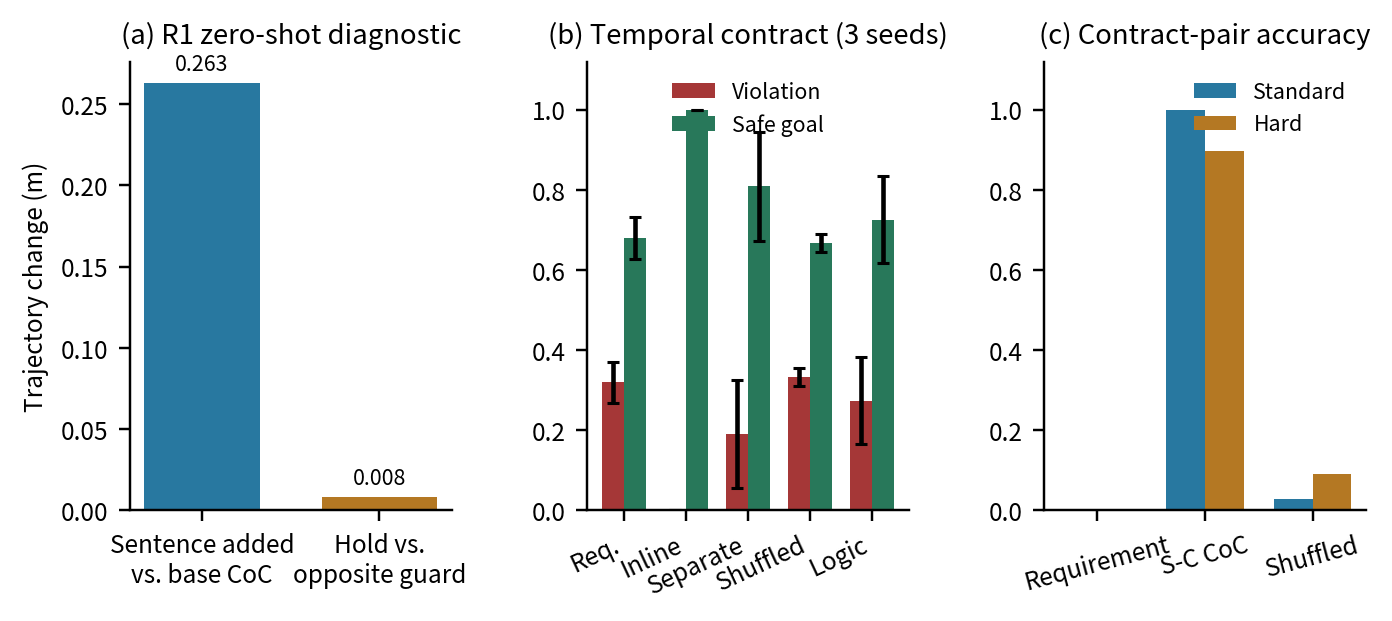
\includegraphics[width=0.95\textwidth]{../latex-kiee-review-2022/figures/fig04_results.png}
\caption{주요 실험 결과의 요약.}
\label{fig:results}
\end{figure*}

\subsection{폐루프 보조 결과}

모든 주행 단계를 포함한 학습 자료에 정지 후 대기 전이 1,404개를 추가하자, 상태 전용, 상태+CoC, 동적 계약 및 단조 단계 계약 조건 모두 300회 평가에서 정지 구간 조기 진입이 발생하지 않았다. 분포 밖 상황의 가드 위반률은 상태 전용 2.6\%, 상태+CoC 1.4\%, 동적 계약, 단조 단계 계약 및 계약+차단장치 조건은 모두 0\%였다. 이미 학습 자료만으로 해결된 조건에서 실행 차단 장치는 위반률을 더 낮추지 못한 채 주행당 평균 2.539회 개입하였다. 이는 충분한 성공 시연이 누락된 제약 일부를 암묵적으로 보완할 수 있고, 불필요한 차단은 진행을 방해하는 비용을 만들 수 있음을 보여준다.

반면 학습에서 보지 못한 해제 후 재위험 상황에서는 가드 위반률이 상태 전용 46.6\%, 상태+CoC 48.6\%, 동적 계약 21.4\%, 단조 단계 계약 37.9\%, 계약+차단장치 4.8\%였다. 모든 조건의 목표 완료율은 100\%였다. 앞으로 1.2초 동안의 상황을 완벽히 안다고 가정한 비현실적 상한선만 위반률 0\%를 달성하였다. 계약 정보가 실제 상황보다 0.4초 늦게 도착하면 동적 계약은 48.1\%, 계약+차단장치는 34.8\%로 악화되었다. 따라서 학습된 계약도 학습하지 않은 단계 전환, 위험 요소의 재등장 및 늦게 갱신된 계약까지 안전하게 처리한다고 보장할 수 없다.

\begin{figure*}[t]
\centering
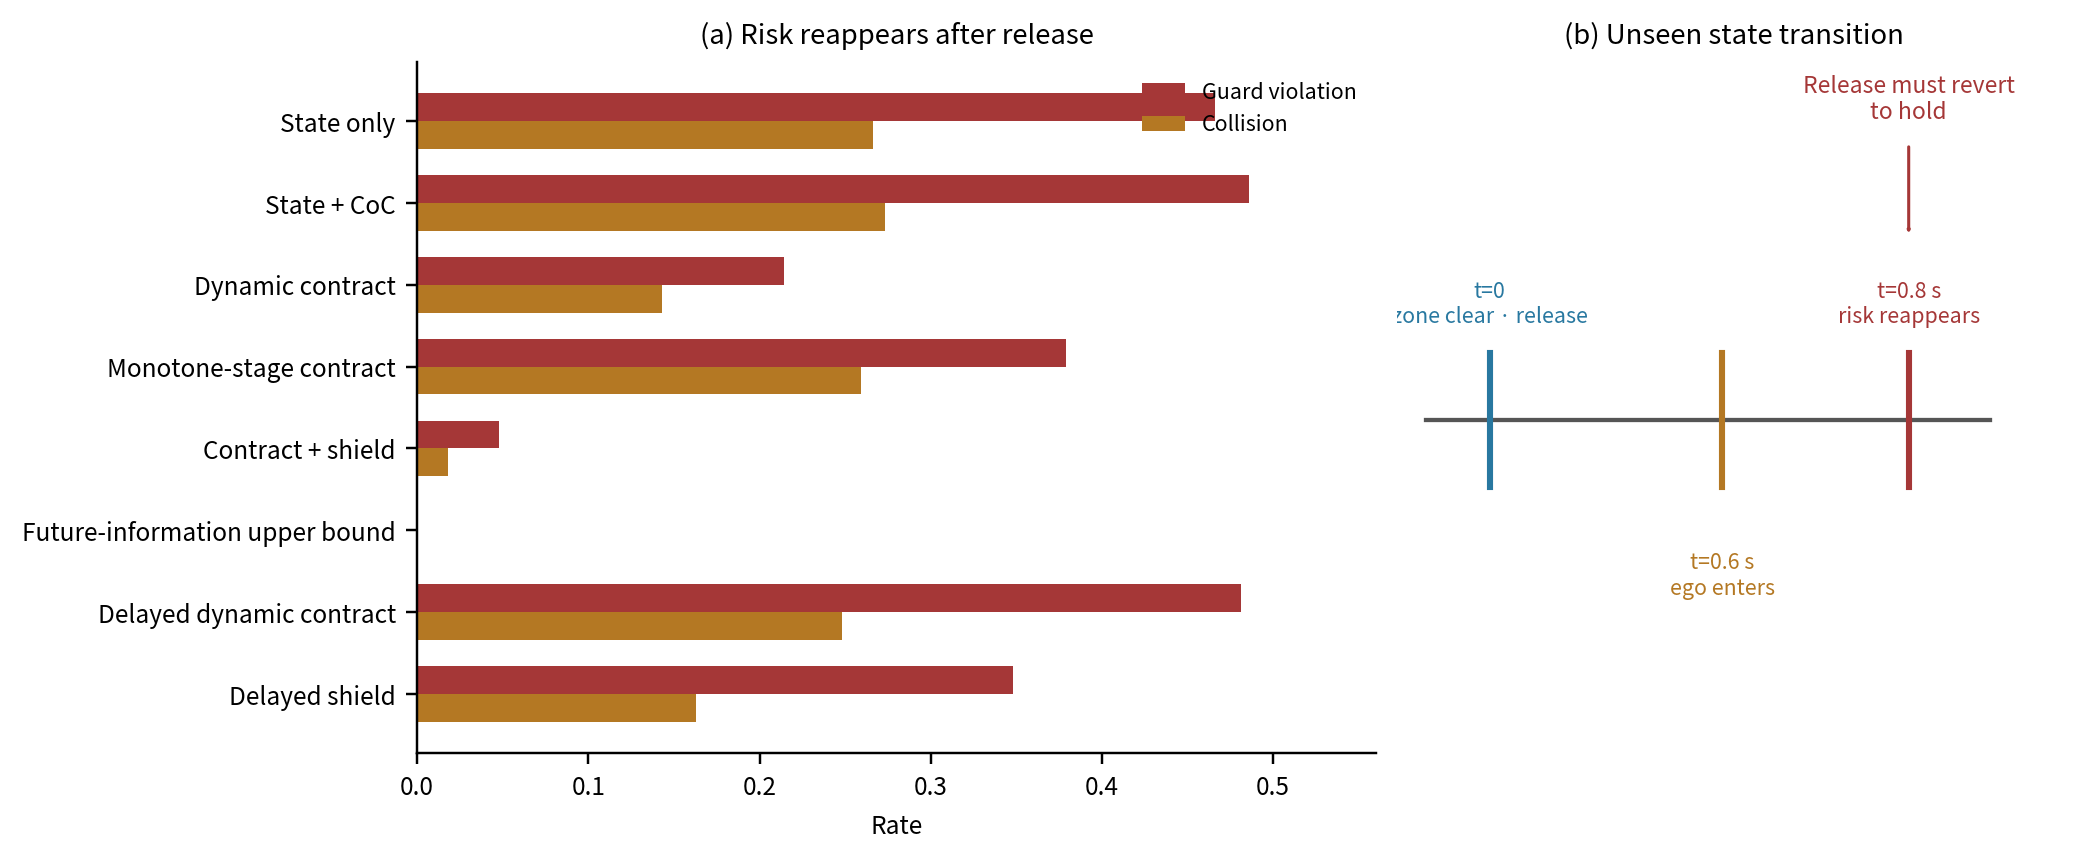
\includegraphics[width=0.91\textwidth]{../latex-kiee-review-2022/figures/fig06_release_reversal.png}
\caption{폐루프 release-reversal stress 결과와 미관측 $\mathrm{RELEASED}\rightarrow\mathrm{HOLD}$ 전이. Oracle은 배포 가능한 방법이 아니라 미래 예측의 상한선이다.}
\label{fig:release-reversal}
\end{figure*}
% Historical, uncompiled duplicate. The current experimental setup and results
% are integrated into sections/05-experiments.tex and main.tex intentionally
% does not input this file.
